\documentclass{scrartcl}
\usepackage[utf8]{inputenc}
\usepackage{scrlayer-scrpage}
\usepackage[czech]{babel}
\usepackage{amsmath}
\usepackage{graphicx}


\cohead[Automaty a gramatiky]
        {Automaty a gramatiky}
\lohead[Úkol č. 4]
        {Úkol č. 4}
\rohead[Václav Luňák]
        {Václav Luňák}
\pagestyle{plain.scrheadings}

\graphicspath{ {.} }

\begin{document}
    \section{}
    
    Mějme pro jazyk $L$ konečný deterministický automat $A = (Q, \Sigma, \delta, q_0, F)$. Pro každý stav $q \in Q$ uděláme následující:
    \begin{itemize}
        \item Nejprve rozdělíme $A$ na části $A_1$ a $A_2$, přičemž v $A_1$ budou stavy, ze kterých je dosažitelné $q$ a v $A_2$ stavy, které jsou dosažitelné z $q$. Jelikož některé stavy mohou být v obou částech, tato operace nám může potenciálně až zdvojnásobit počet stavů.
        \begin{center}
            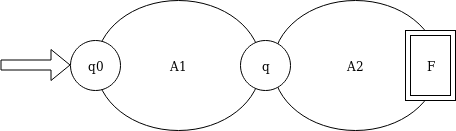
\includegraphics[width=250pt]{automaty_4_1.png}
        \end{center}
        \item Poté automat přestavíme následujícím způsobem:
        \begin{center}
            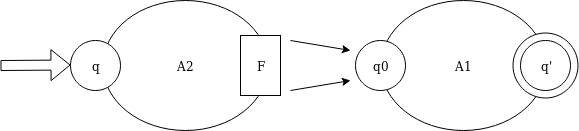
\includegraphics[width=250pt]{automaty_4_2.png}
        \end{center}
        Ze všech stavů $F$ vedou $\lambda$-přechody do $q_0$ a na pozici $q$ v $A_1$ je nově stav $q'$. Navíc stavy $F$ nejsou přijímající; jediným přijímajícím stavem je $q'$ \\

        Uvědomme si, že tento automat přijímá právě slova, která jsou "zalomená v $q$"; tj. $\{yx | xy \in L, \delta^*(q_0, x) = q\}$. To vypozorujeme snadno z konstrukce automatu. Správná slova automat přijme očividně: z $q$ do $F$ se dostane, jelikož $\delta^*(q, y)$ musí být přijímající stav, a z $q_0$ do $q$ (resp. do $q'$) se dostane z definice množiny. \\

        Máme-li naopak slovo $w$ mimo tuto množinu, automat ho nepřijme. Kdyby ano, muselo by $w = yx$ tak, že $\delta^*(q,x) \in F$, jinak se nemůžeme dostat přes prví část automatu. Navíc by muselo platit $\delta^*(q0, x) = q$, jelikož $q'$ je na původní pozici $q$ a je to jediný přijímající stav automatu. Tím máme ale spor s tím, že $w$ nenáleží naší množině.
    \end{itemize}

    Vytvořili jsme tedy $\vert Q \vert$ takovýchto automatů, jeden pro každý stav $A$. Tím nám vznikl nedeterministický konečný automat, který přijímá slova $shift(L)$, neboť pro jakkoliv posunuté slovo dokáže "vybrat" právě automat, který odpovídá tomu danému posunutí.
    Naopak z výše uvedeného žádný dílčí automat nepřijímá jiná slova, tedy je nebude přijímat ani ten výsledný.
\end{document}